Considering the limitations outlined in section
\ref{sssec:mapreduce_limitations}, Vinod Kumar Vavilapalli et
al. presented YARN \cite{Vavilapalli:2013:AHY:2523616.2523633} the new
resource management layer that was adopted in Hadoop 2.0. The new
Hadoop stack now is depicted in Figure \ref{fig:yarn_hadoop1_hadoop2_arch} where YARN is the
cluster resource management module and MapReduce is one out of plenty
applications running on top of YARN. This architectural transformation
paved the way for a wide variety of frameworks like
Apache Spark \cite{apache_spark}, Apache Flink \cite{apache_flink},
Apache Pig \cite{apache_pig}, etc to run on the
Hadoop platform like any other YARN application.

\begin{figure}
\centering
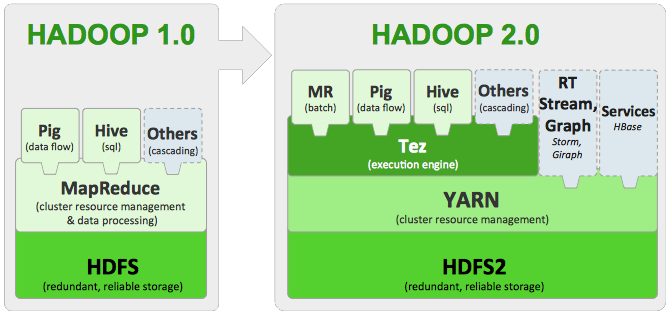
\includegraphics[scale=0.6]{resources/images/Background/hadoop1_hadoop2_arch.png}
\label{fig:yarn_hadoop1_hadoop2_arch}
\caption{Hadoop 2.0 stack \cite{hortonworks_hadoop_stack}}
\end{figure}

The new architecture of Hadoop 2.x separates the resource management
functions from the programming model. It delegates the
intra-application communication and the tracking of the execution flow
to per-job components. That unlocks great performance improvements,
improves scalability and enables a wide variety of frameworks to share
the cluster resources in a very gentle way.

YARN uses three main components to provide a scalable and fault
tolerant resource management platform. The first component is the
\emph{ResourceManager} (RM), a per-cluster daemon that tracks resource
usage and node liveness and schedules jobs on the cluster. The second
component is a per-node \emph{NodeManager} (NM) which is responsible
for monitoring resource availability on the specific node, reporting
faults to RM and managing container life-cycle. Finally, there is the
\emph{ApplicationMaster} (AM) which coordinates the logical plan of a
single job, manages the physical resources offered by the RM and
tracks the execution of the job. A high level overview of YARN
architecture is described in Figure \ref{fig:yarn_arch_overview}. RM
has a global view of the cluster and provides the scheduling
functionality, while the per-job AM manages the dynamic resource
requests and the workflow of the tasks. Containers that are allocated
by the RM are locally managed by the NM in each node in the cluster.

\begin{figure}
\centering
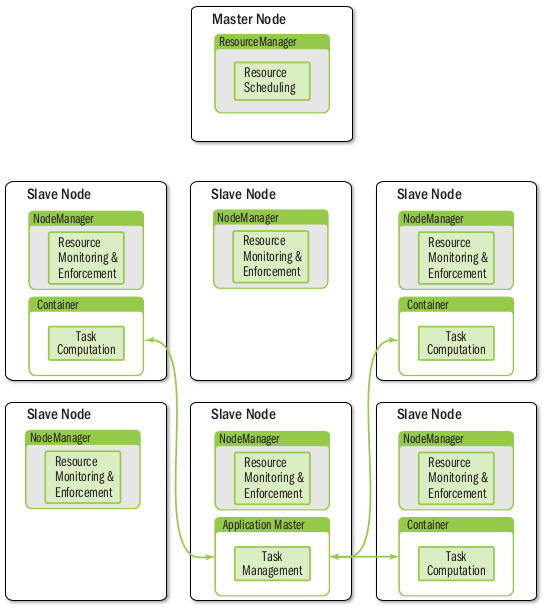
\includegraphics[scale=0.5]{resources/images/Background/yarn_arch_overview.png}
\label{fig:yarn_arch_overview}
\caption{YARN architecture overview \cite{Murthy:2014:AHY:2636998}}
\end{figure}

\subsubsection{ResourceManager}
\label{sssec:rm}
In YARN the RM acts as the central authority for allocating resources
in the cluster. It works closely with the per-node NodeManager getting
an updated view of the cluster by the heartbeats received. The RM
itself allocates generic resources in the cluster in the form of
\emph{containers} that have specific CPU and RAM requirements. Those
resource requests are piggybacked in the heartbeats issued by every AM.
As RM is completely unaware about the job execution plan,
it is up to the AM to make local optimizations and assign the
resources accordingly. RM internally consists of several modules but
the three most important are the \emph{ApplicationMasterService}, the
\emph{ResourceTrackerService} and the \emph{Yarn Scheduler} as shown
in Figure \ref{fig:yarn_RM_components}.

\begin{figure}
\centering
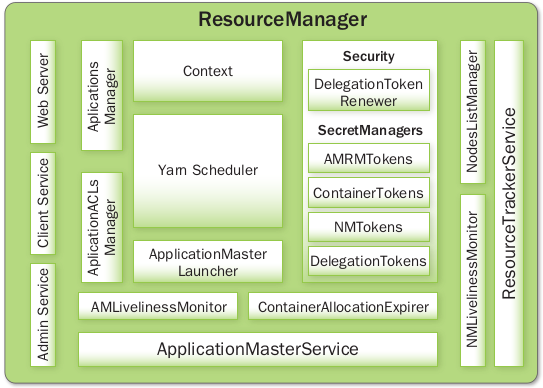
\includegraphics[scale=0.5]{resources/images/Background/RM_components.png}
\label{fig:yarn_RM_components}
\caption{ResourceManager components \cite{Murthy:2014:AHY:2636998}}
\end{figure}

The \emph{ApplicationMasterService} is responsible for receiving and
handling heartbeats from the AMs that are launched in the
cluster. Heartbeats are designed to be as compact as possible, still
not excluding any vital information. For that reason, Google Protocol
Buffers \cite{proto_buf} are used for every communication among YARN
components. Protocol Buffers is a language-neutral, platform-neutral
mechanism for efficiently serializing data. The heartbeat mechanism
serves both as a scalable way for the RM and AM to communicate, but
also for the RM to track the liveness of AMs. \emph{ResourceRequests}
contain information such as the resources per container in terms of
virtual cores and memory, the number of containers, locality
preferences and priority of requests. The scheduler then tracks,
updates and satisfies these requests with available resources in the
cluster. The RM builds the view of the cluster with the available
resources from the information it receives from the NMs. The scheduler
tries to match the locality constraints as much as possible and
responds back to AM with the allocated containers along with
credentials that grant access to them. The RM also keeps track of the
AM health through the heartbeats received. The component that handle
the liveness property of every AM is the \emph{AMLivenessMonitor}. In
case of a missed heartbeat, that particular AM is deemed dead and
is expired by the RM. All the containers that were allocated for
that AM are marked as dead and the RM reschedules the same application
(ApplicationMaster) on a new container.

As I have previously mentioned, the RM builds its view of the cluster
by the information that NMs send to it. The
\emph{ResourceTrackerService} component is responsible for handling such RPCs
and forwarding them to the appropriate modules. Before a new node in the
cluster is able to execute YARN jobs, it should first register itself
with the RM through the ResourceTrackerService and exchange some
security tokens. A heartbeat mechanism is also used in this place to
ensure the liveness of NMs and to receive updated information about
the available resources in the physical machine. The newly received
information about the available resources on that node is forwarded to the YARN
scheduler so it can make scheduling decisions. Also, a received
heartbeat is forwarded to the \emph{NMLivelinessMonitor} module which
keeps track of the health of NMs. If RM has not received any heartbeat
from a NM after a configurable timeout, then it is deemed dead and is
expired. All the containers that were currently running on that node
are also marked as dead and an event is sent to the scheduling module
not to schedule any job on that node. When the node restarts, it
registers again with the RM and it makes itself available for
scheduling again.

At the core of RM is the \emph{YarnScheduler} that is responsible of
making scheduling decisions based on the available resources on the
cluster and the resource requests issued by the AMs. Currently the
resource requirements of an AM are limited to the number of virtual
cores and to the amount of memory a container should
have. YarnScheduler is a pluggable module and at the time of writing
there are three different options. The first and original option is
the \emph{FIFO Scheduler} where jobs are served in a simple
first-in-first-out order with no sense of priorities. The second
scheduling policy is the \emph{Capacity Scheduler}
\cite{capacity_scheduler} developed by Yahoo! Capacity Scheduler
is primarily built for large clusters with resources that are shared
among different units in the same organization. There are different
queues serving jobs for various units while guaranteeing some minimum
capacity for each queue. Any excess capacity can be temporarily
allocated to other queues and a job with high priority will be executed
before any other job with lower priority. If a job cannot be scheduled
in its respective queue due to lack of resources and that queue is
below its fair share, then jobs in other queues can be preempted. Last
but not least is the \emph{Fair Scheduler} \cite{fair_scheduler}
developed by Facebook. In Fair Scheduler every application belongs to
a queue, by default the ``default'' queue. The basic idea is that
containers are allocated to the application with the fewer resources
assigned within the queue, providing a uniform distribution of the
available cluster resources in the long run. There can be multiple
queue with support for priorities, minimum and maximum shares and FIFO
ordering within the queue. Similar to Capacity Scheduler, Fair Scheduler
also has support for preemption of containers that are already
assigned. Currently the default scheduler for Hadoop is the Capacity Scheduler.

\subsubsection{ApplicationMaster}
\label{sssec:am}
Upon a successful submission of an application to RM, the latter
creates a special container in a node called
\emph{ApplicationMaster}. AM is a per-application process that
coordinates the execution plan of the application, negotiates
resources with the RM and monitors the assigned containers. AM
periodically heartbeats RM, default value is 10 minutes, to prove it
is alive and to dynamically request more resources or release
some. When AM is launched, it will compute the necessary requirements
and locality preferences, encode them and through the heartbeat
mechanism send them to RM. RM depending on the scheduling decisions it
has made it might respond back with any empty response or with
\emph{container leases} on different nodes. AM will contact the
respective NodeManagers, present them the leases and the NM will
create the containers. Afterwards, it (AM) is responsible to monitor the liveness
of the containers or implement any recovery functions. An overview of
the workflow explained above is illustrated in Figure \ref{fig:yarn_am_rm_interaction}.

\begin{figure}
\centering
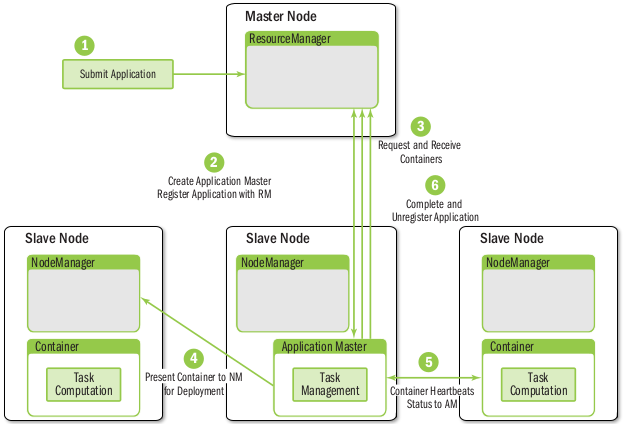
\includegraphics[scale=0.6]{resources/images/Background/AM_RM_interaction.png}
\label{fig:yarn_am_rm_interaction}
\caption{ApplicationMaster interaction \cite{Murthy:2014:AHY:2636998}}
\end{figure}

Since a key requirement for YARN was to decouple the programming model
from the resource management, AM is not tightly connected to YARN.
Writing an ApplicationMaster process is not an easy task but Hadoop
offers some APIs to avoid the complexity of low-level protocols.
Users can write their own ApplicationMaster
process fitting particular needs of making local optimizations with
the containers allocated by the RM, monitoring the containers,
define the recovery procedures when a container dies or capture the
exit status of a finished task. That opened the road for a plethora
of applications to run on Hadoop such as Apache Spark
\cite{apache_spark}, Apache Flink \cite{apache_flink}, Apache Hadoop
MapReduce \cite{apache_hadoop} etc.

\subsubsection{NodeManager}
\label{sssec:nm}
The \emph{NodeManager} is the ``worker'' daemon that runs on every
physical node of a Hadoop cluster. It is responsible for monitoring
the health of the physical hardware, authenticating the container
leases, preparing, monitoring and tearing down the container and
providing a set of services to the application.

When a node joins a cluster, the NM should register with the
RM. It will present the total amount of virtual cores and memory
available in this machine, some security tokens required to
authenticate the container leases, some communication ports etc. From
that point NM should periodically heartbeat the RM, default value is 1
second, proving that is still alive and keeping the RM up-to-date with
its status. NM regularly runs some monitoring scripts for the
health of the machine and the status is sent to RM. As a response it
might get back a list of container leases or some instructions such as
node decommission because of unhealthy node or to kill some
containers. In case of a missed heartbeat, the RM declares the NM as
dead, excludes that node from its pool of resources and informs all
running AMs about the failed NM. AM is responsible to react to such a
failure and possibly ask resources from RM to redo the work done in
the failed node.

Each container in YARN comes along with a \emph{container launch
  context} (CLC). The CLC contains information specific to the
application that is about to run such as environment variables,
dependencies stored in HDFS or on-line, security tokens, commands that
actually spawn the application etc. Once the NM has validated the
container lease with the security tokens provided, it should
initialize the container by fetching the requested dependencies,
setting the variables and of course run the commands specified by the
CLC. At the end of the container life-cycle or if the container dies
or if RM instructs NM to kill a container, NM should garbage collect
any dependency fetched during initialization and not used any
longer by other containers in that node. For the whole duration of a
container's life-cycle, NM monitors its utilization. If a container's
usage exceeds its assigned, then the NM signals the container to be
killed so that it does not disrupt the work of other containers
sharing the same physical machine. 

Finally, NM provides some services to the containers such as log
aggregation that will upload anything written to \texttt{stdout} or \texttt{stderr} to
HDFS when the application finishes. NM also provides a set of
auxiliary, pluggable services that are used by some applications. For
example, in MapReduce the intermediate output of the Map phase should
not be garbage collected after the container has finished. The
service will flag these data to be persisted even after the container
has gracefully exit.

\subsubsection{YARN fault tolerance \& HA}
\label{sssec:yarn_ha}
So far we have gone through some key points of the resource management
platform of Hadoop. RM is the central authority that makes scheduling
decisions and carries all the burden of monitoring both the AMs and
the NMs. Although from the beginning Hadoop was designed to run on
commodity hardware were machine failures are the norm, a
ResourceManager failure would drove the whole cluster
useless. Moreover, after a RM restart, it had to kill all the
containers running on the cluster including the ApplicationMasters and
launch new instances of them. Since RM is not responsible for the
recovery of the applications AMs had to start over the jobs, unless if
they had some recovery policy. Hadoop 2.4 introduced some kind of recovery mechanism that would
recover some application metadata and re-submit only the non-finished
applications in a way invisible to the user. As of Hadoop 2.6 RM
restart has further improved. The rest of this section will briefly
explain the recovery and HA mechanism of the RM.

To recover from a failure, RM needs to
store some state in a persistent storage. Currently there is support
for three alternatives. The first one is to use the Apache ZooKeeper
\cite{apache_zookeeper}, a service that provides highly reliable
distributed coordination, naming, storing and group membership
services. The second alternative is LevelDB \cite{google_leveldb},
a light-weight key-value store and finally the local file system or
HDFS. The default state store is the file system, local or HDFS, although
if a requirement of our cluster is also HA, then Apache ZooKeeper is
the preferred one. To begin with, RM store some application metadata to
the persistent storage solution. These metadata include the
application submission context, the final status of the application,
diagnostics of the application and some security related
tokens. Moreover, when the RM restarts it will ask from all the NMs in
the cluster to re-sync and send back information about all the
containers that are currently running. Using that information it can
recover the whole state of the scheduler such as resource requests,
queues' usage etc. That way RM does not need to kill and kick-off again all
the running applications, just instruct the respective AMs to re-sync
with it.

Even with the aforementioned mechanism RM is a single point of
failure. In case of an RM crash, the cluster would be useless until
the RM restarts and recover. This period, depending on the number of
nodes on the cluster, the number of applications running and the
policies to detect a dead machine, might take quite a long time. As of
Hadoop 2.4 there is a High Availability feature for the RM, using an
Active/Standby architecture and a ZooKeeper instance to coordinate
the RM nodes. ZooKeeper
ensures that at any point of time there is only one Active node that
performs all the work. In case of a crash, a new leader is elected
from the Standby pool and is promoted to Active. The transition from
Standby to Active can be done either manually through the administration
CLI or automatically where ZooKeeper will detect the crashed node and
elect a new leader. The new Active RM will build the current state
from the state stored in ZooKeeper. AMs and NMs will keep contacting
the crashed, previously Active, RM until they realize it is dead. Then
they will contact the next RM in their configuration list until they
hit the currently Active node in a round-robin fashion.
